\documentclass[tikz]{standalone}
\usepackage{tikz}
\usetikzlibrary{positioning}

\begin{document}
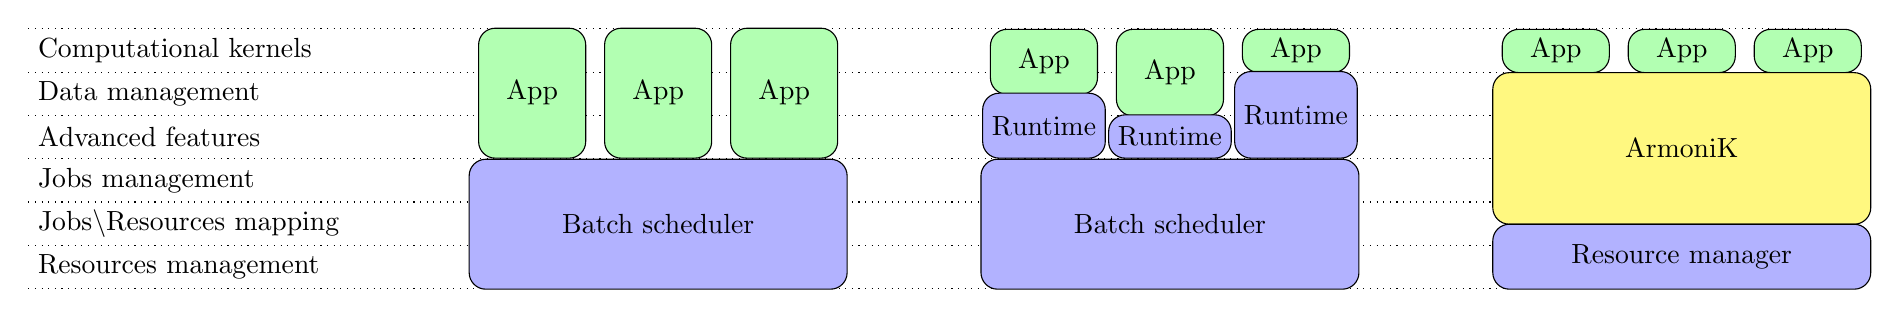
\begin{tikzpicture}[rounded corners=2pt]

% Sizes
\def\appw{1.6}
\def\apph{0.55}
\def\gap{0.85}

% Add some dotted lines as guide
\foreach \y in {5, 4, 3, 2, 1, 0, -1} {
    \draw[dotted] (-8,\y*\apph) -- (15,\y*\apph);
}

% Scheduler properties
\foreach \i/\text in {
5/Computational kernels,
4/Data management,
3/Advanced features,
2/Jobs management,
1/Jobs\textbackslash Resources mapping,
0/Resources management
} {
  \node[anchor=west] at (-8,\i*\apph - 0.5*\apph ) {\text};
}

% Batch only
\foreach \i in {-1,0,1} {
  \node[draw, fill=green!30, minimum width=\appw*\gap cm, minimum height=3 * \apph cm, anchor=south, rounded corners=6pt]
        at (\i*\appw,2*\apph) {App};
}
\node[draw, fill=blue!30, minimum width=3 * \appw cm, minimum height=3 * \apph cm, anchor=north, rounded corners=6pt]
      at (0,2*\apph) {Batch scheduler};

% Batch + Runtime
\node[draw, fill=green!30, minimum width=\appw*\gap cm, minimum height=1.5 * \apph cm, anchor=north, rounded corners=6pt]
        at (-1 * \appw + 6.5,5 * \apph) {App};
\node[draw, fill=blue!30, minimum width=\appw*\gap cm, minimum height=1.5 * \apph cm, anchor=south, rounded corners=6pt]
        at (-1 * \appw + 6.5,2 * \apph) {Runtime};

\node[draw, fill=green!30, minimum width=\appw*\gap cm, minimum height=2*\apph cm, anchor=north, rounded corners=6pt]
        at (0 * \appw + 6.5,5 * \apph) {App};
\node[draw, fill=blue!30, minimum width=\appw*\gap cm, minimum height=\apph cm,, anchor=south, rounded corners=6pt]
        at (0 * \appw + 6.5,2 * \apph) {Runtime};

\node[draw, fill=green!30, minimum width=\appw*\gap cm, minimum height=\apph cm, anchor=north, rounded corners=6pt]
        at (1 * \appw + 6.5,5 * \apph) {App};
\node[draw, fill=blue!30, minimum width=\appw*\gap cm, minimum height=2*\apph cm,, anchor=south, rounded corners=6pt]
        at (1 * \appw + 6.5,2 * \apph) {Runtime};

\node[draw, fill=blue!30, minimum width=3 * \appw cm, minimum height=3 * \apph cm, anchor=north, rounded corners=6pt]
      at (6.5,2 * \apph) {Batch scheduler};

% ArmoniK + Resource Manager
\foreach \i in {-1,0,1} {
  \node[draw, fill=green!30, minimum width=\appw*\gap cm, minimum height=\apph cm, anchor=north,rounded corners=6pt]
        at (\i*\appw + 13, 5 * \apph) {App};
}
\node[draw, fill=yellow!50, minimum width=3 * \appw cm, minimum height=3.5 * \apph cm, anchor=north, rounded corners=6pt]
      at (13,4 * \apph) {ArmoniK};
\node[draw, fill=blue!30, minimum width=3 * \appw cm, minimum height=1.5 * \apph cm, anchor=north, rounded corners=6pt]
      at (13,0.5 * \apph) {Resource manager};

\end{tikzpicture}
\end{document}
